\subsection*{Paso 1: inicialización}

Inicialmente, todos los flujos son cero:

\begin{center}
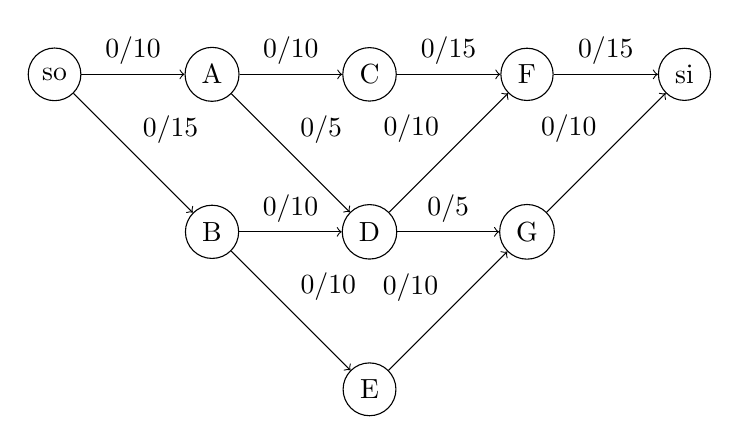
\begin{tikzpicture}[node distance=2cm, auto]
    \node[draw, circle] (so) {so};
    \node[draw, circle, right of=so] (A) {A};
    \node[draw, circle, below of=A] (B) {B};
    \node[draw, circle, right of=A] (C) {C};
    \node[draw, circle, below of=C] (D) {D};
    \node[draw, circle, below of=D] (E) {E};
    \node[draw, circle, right of=C] (F) {F};
    \node[draw, circle, below of=F] (G) {G};
    \node[draw, circle, right of=F] (si) {si};
    
    % Edges with capacities
    \draw[->] (so) -- node {0/10} (A);
    \draw[->] (so) -- node {0/15} (B);
    \draw[->] (A) -- node {0/10} (C);
    \draw[->] (A) -- node {0/5} (D);
    \draw[->] (B) -- node {0/10} (D);
    \draw[->] (B) -- node {0/10} (E);
    \draw[->] (C) -- node {0/15} (F);
    \draw[->] (D) -- node {0/10} (F);
    \draw[->] (D) -- node {0/5} (G);
    \draw[->] (E) -- node {0/10} (G);
    \draw[->] (F) -- node {0/15} (si);
    \draw[->] (G) -- node {0/10} (si);
\end{tikzpicture}
\end{center}

\subsection*{Paso 2: primer camino de aumento}

Seleccionamos el camino \(so \rightarrow B \rightarrow D \rightarrow F \rightarrow si\). el flujo de aumento es \(\min(15, 10, 10, 15) = 10\).

\begin{center}
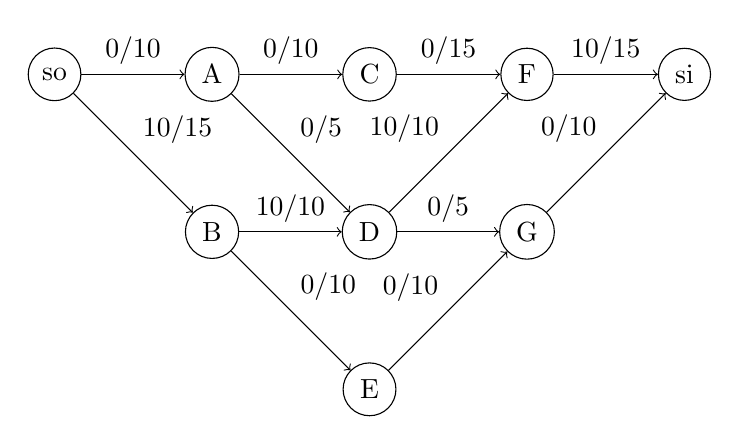
\begin{tikzpicture}[node distance=2cm, auto]
    \node[draw, circle] (so) {so};
    \node[draw, circle, right of=so] (A) {A};
    \node[draw, circle, below of=A] (B) {B};
    \node[draw, circle, right of=A] (C) {C};
    \node[draw, circle, below of=C] (D) {D};
    \node[draw, circle, below of=D] (E) {E};
    \node[draw, circle, right of=C] (F) {F};
    \node[draw, circle, below of=F] (G) {G};
    \node[draw, circle, right of=F] (si) {si};
    
    % Edges with capacities and flows
    \draw[->] (so) -- node {0/10} (A);
    \draw[->] (so) -- node {10/15} (B);
    \draw[->] (A) -- node {0/10} (C);
    \draw[->] (A) -- node {0/5} (D);
    \draw[->] (B) -- node {10/10} (D);
    \draw[->] (B) -- node {0/10} (E);
    \draw[->] (C) -- node {0/15} (F);
    \draw[->] (D) -- node {10/10} (F);
    \draw[->] (D) -- node {0/5} (G);
    \draw[->] (E) -- node {0/10} (G);
    \draw[->] (F) -- node {10/15} (si);
    \draw[->] (G) -- node {0/10} (si);
\end{tikzpicture}
\end{center}

% Capacidades residuales:
% - \(so \rightarrow B: 5\)
% - \(B \rightarrow D: 0\)
% - \(D \rightarrow F: 0\)
% - \(F \rightarrow si: 5\)

\subsection*{Paso 3: segundo camino de aumento}

Seleccionamos el camino \(so \rightarrow A \rightarrow C \rightarrow F \rightarrow si\). el flujo de aumento es \(\min(10, 10, 15, 5) = 5\).

\begin{center}
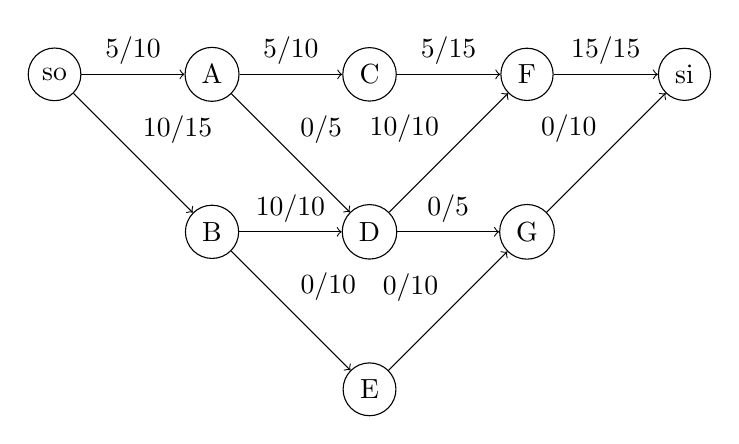
\begin{tikzpicture}[node distance=2cm, auto]
    \node[draw, circle] (so) {so};
    \node[draw, circle, right of=so] (A) {A};
    \node[draw, circle, below of=A] (B) {B};
    \node[draw, circle, right of=A] (C) {C};
    \node[draw, circle, below of=C] (D) {D};
    \node[draw, circle, below of=D] (E) {E};
    \node[draw, circle, right of=C] (F) {F};
    \node[draw, circle, below of=F] (G) {G};
    \node[draw, circle, right of=F] (si) {si};
    
    % Edges with capacities and flows
    \draw[->] (so) -- node {5/10} (A);
    \draw[->] (so) -- node {10/15} (B);
    \draw[->] (A) -- node {5/10} (C);
    \draw[->] (A) -- node {0/5} (D);
    \draw[->] (B) -- node {10/10} (D);
    \draw[->] (B) -- node {0/10} (E);
    \draw[->] (C) -- node {5/15} (F);
    \draw[->] (D) -- node {10/10} (F);
    \draw[->] (D) -- node {0/5} (G);
    \draw[->] (E) -- node {0/10} (G);
    \draw[->] (F) -- node {15/15} (si);
    \draw[->] (G) -- node {0/10} (si);
\end{tikzpicture}
\end{center}

% Capacidades residuales:
% - \(so \rightarrow A: 5\)
% - \(A \rightarrow C: 5\)
% - \(C \rightarrow F: 10\)
% - \(F \rightarrow si: 0\)

\subsection*{Paso 4: tercer camino de aumento}

Seleccionamos el camino \(so \rightarrow A \rightarrow D \rightarrow G \rightarrow si\). el flujo de aumento es \(\min(5, 5, 5, 10) = 5\).

\begin{center}
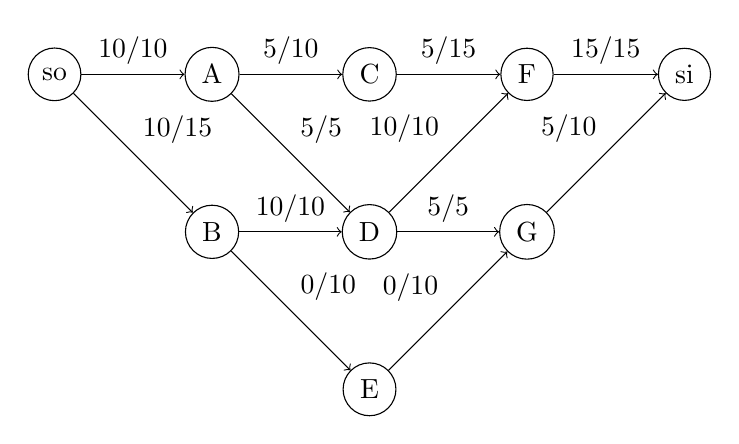
\begin{tikzpicture}[node distance=2cm, auto]
    \node[draw, circle] (so) {so};
    \node[draw, circle, right of=so] (A) {A};
    \node[draw, circle, below of=A] (B) {B};
    \node[draw, circle, right of=A] (C) {C};
    \node[draw, circle, below of=C] (D) {D};
    \node[draw, circle, below of=D] (E) {E};
    \node[draw, circle, right of=C] (F) {F};
    \node[draw, circle, below of=F] (G) {G};
    \node[draw, circle, right of=F] (si) {si};
    
    % Edges with capacities and flows
    \draw[->] (so) -- node {10/10} (A);
    \draw[->] (so) -- node {10/15} (B);
    \draw[->] (A) -- node {5/10} (C);
    \draw[->] (A) -- node {5/5} (D);
    \draw[->] (B) -- node {10/10} (D);
    \draw[->] (B) -- node {0/10} (E);
    \draw[->] (C) -- node {5/15} (F);
    \draw[->] (D) -- node {10/10} (F);
    \draw[->] (D) -- node {5/5} (G);
    % \draw[->] (E) -- node {0/10};
    \draw[->] (E) -- node {0/10} (G);
    \draw[->] (F) -- node {15/15} (si);
    \draw[->] (G) -- node {5/10} (si);
\end{tikzpicture}
\end{center}

% Capacidades residuales:
% - \(so \rightarrow A: 0\)
% - \(A \rightarrow D: 0\)
% - \(D \rightarrow G: 0\)
% - \(G \rightarrow si: 5\)

\subsection*{Paso 5: cuarto camino de aumento}

Seleccionamos el camino \(so \rightarrow B \rightarrow E \rightarrow G \rightarrow si\). el flujo de aumento es \(\min(5, 10, 10, 5) = 5\).

\begin{center}
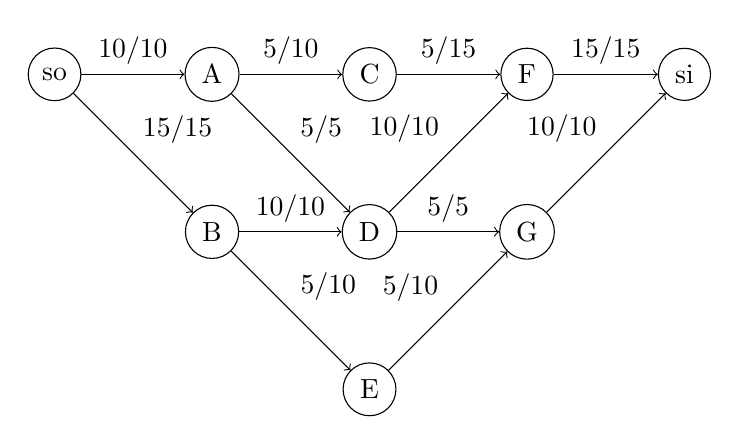
\begin{tikzpicture}[node distance=2cm, auto]
    \node[draw, circle] (so) {so};
    \node[draw, circle, right of=so] (A) {A};
    \node[draw, circle, below of=A] (B) {B};
    \node[draw, circle, right of=A] (C) {C};
    \node[draw, circle, below of=C] (D) {D};
    \node[draw, circle, below of=D] (E) {E};
    \node[draw, circle, right of=C] (F) {F};
    \node[draw, circle, below of=F] (G) {G};
    \node[draw, circle, right of=F] (si) {si};
    
    % Edges with capacities and flows
    \draw[->] (so) -- node {10/10} (A);
    \draw[->] (so) -- node {15/15} (B);
    \draw[->] (A) -- node {5/10} (C);
    \draw[->] (A) -- node {5/5} (D);
    \draw[->] (B) -- node {10/10} (D);
    \draw[->] (B) -- node {5/10} (E);
    \draw[->] (C) -- node {5/15} (F);
    \draw[->] (D) -- node {10/10} (F);
    \draw[->] (D) -- node {5/5} (G);
    \draw[->] (E) -- node {5/10} (G);
    \draw[->] (F) -- node {15/15} (si);
    \draw[->] (G) -- node {10/10} (si);
\end{tikzpicture}
\end{center}

% Capacidades residuales:
% - \(so \rightarrow B: 0\)
% - \(B \rightarrow E: 5\)
% - \(E \rightarrow G: 5\)
% - \(G \rightarrow si: 0\)

El corte que separa el nodo \(so\) del resto del grafo es un corte con capacidad residual 0.

El flujo máximo total es \(25\) l/min.

